\chapter{Optimization}
This chapter will examine optimization possibilities on the final product as described in \textbf{XX}. There are multiple ways of optimizing a product, but this chapter will only examine the options which could have been implemented, but due to time constraints are not. 

\subsection*{Instructions}
The amount of instructions per sample on average is \textbf{XX}, which could have been optimized significantly. This could be done by avoiding calls as they take 10 clock cycles \todo{REF} because the pipeline has to be emptied. In the system, calls are used many places where it is unnecessarily. They were implemented as they give an easier overview of the system. By removing the calls the amount of instructions will be reduced. 

An example of optimizing the software is the use of buffers in the software for example downFunc() which is described in \textbf{XX}. In downFunc() samples are firstly loaded into a buffer and then afterwards loaded into another buffer used for the FIR filter. This means that two identical buffers need to be initialized instead of one which will reduce the complexity of the software and the number of instructions. 

Another example is the use of internal resources in the DSP. Firstly, the DSP has five internal circular buffers but in the software only one circular buffer is used, which means that the same circular buffer is initialized every time it is used. A better solution would be using all five circular buffers such that the amount of initialization is reduced. Secondly, the DSP is capable of performing parallel execution such as one dual MAC per clock cycle. This is neither used in the FIR routine, where it would reduce the repeats of the MAC by two, which means that the amount of computation needed for the filter algorithm is halved.  

\subsubsection*{Polyphase FIR filter}
The algorithm of the interpolation in the system is to insert a 0 in between each sample and the filter the output. By not multiply-accumulate with zero, the amount of computation to perform the interpolation algorithm is halved. This can be achieved by the use of polyphase filters. The polyphase filter works by dividing the FIR filter coefficients into two sections and then only apply one of the sections to the input when a sample is read. At the next sample the coefficient sections are switched. By doing so, no zero padding is needed and no multiply-accumulate with zero is performed.

\subsubsection*{Sampling the impulse response}
The anti-aliasing filter are designed by using the Kaiser window method where pass-band and stop-band requirement are defined. Another solution is to design the filter by using window method and fix the cutoff frequency to $\frac{fs}{4}$. By doing so, half of the samples of the impulse response are 0 and would therefore half the amount of computation for the decimation filter.



% By using window method the frequency response is not affected because of spectral inversion which makes the frequency reponse flat.

%\subsubsection*{Using IIR filter in interpolation}
% Phase response first gets non-linear at one decade below the cutoff frequency. 
% Non-linear phase do not affect the frequency response as the group delay is only non constant above the bandwidth.


\subsection*{Delay}
The final product has a delay of \textbf{XX} which was concluded to be to high as described in test \textbf{XX} therefore this delay should be reduced. There are several ways of reducing the current delay, such as reducing the orders of the filters, by either moving the filters or by having a smaller attenuation, or by removing octave bands, which leads to larger filter orders but smaller delays because there are less downsamples. By removing an octave band the filters would have to be moved one octave down, which means the filter order would double but it would then be possible to downsample by more than two which would make the filter order small again.

Another possibility of reducing the delay substantially is by converting the interpolation filter from FIR to IIR. It is not possible to convert the decimation filter to IIR because of an non constant group delay which would give an error when summing the signal, but the bandwidth of the interpolation filter is much higher than the bandwidth of decimated signal and therefore the group delay would not be a problem because it is constant approximately until the cutoff frequency of the filter. The IIR filter would have a much lower delay which would in term divide the delay by two.   

\subsection*{RMS Limiter}
The RMS limiters implemented have a small attack time, meaning fast transients will not be caught by the limiter. By implemented a delay as shown in \autoref{fig:optimizationDelay} the RMS limiter have time to detect transients and therefore protect the loudspeaker even better. 
\begin{figure}[H]
\centering
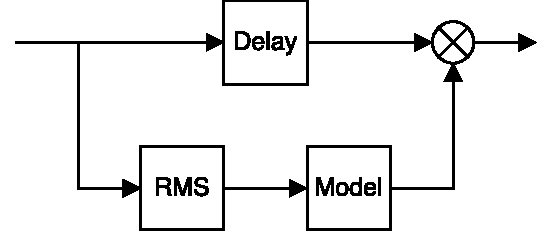
\includegraphics[width=0.4\textwidth]{figures/optimizationDelay.pdf}
\caption{Adding a delay will make the system able to limit transients.}
\label{fig:optimizationDelay}
\end{figure}
By implementing the delay, a peak-limiter is no longer needed to catch transients.



